
\documentclass[a4paper,10pt]{article}

\usepackage[utf8x]{inputenc}
\usepackage[textwidth=170mm,textheight=229mm]{geometry}
\usepackage{graphicx}
\usepackage{amsmath}
\usepackage{fancybox}
\usepackage{cancel}
\usepackage{wrapfig}
\usepackage{amsmath,amssymb,amsfonts,mathrsfs}
\usepackage{color}
\usepackage{slashed}
\usepackage{bbm}  
\usepackage{xspace}
\usepackage{subcaption}
\usepackage{multicol}
\usepackage{tikz}
\usetikzlibrary{arrows,shapes}
\usetikzlibrary{trees}
\usetikzlibrary{matrix,arrows} 				% For commutative diagram
											% http://www.felixl.de/commu.pdf
\usetikzlibrary{positioning}				% For "above of=" commands
\usetikzlibrary{calc,through}				% For coordinates
\usetikzlibrary{decorations.pathreplacing}  % For curly braces
% http://www.math.ucla.edu/~getreuer/tikz.html
\usepackage{pgffor}							% For repeating patterns

\usetikzlibrary{decorations.pathmorphing}	% For Feynman Diagrams
\usetikzlibrary{decorations.markings}
\tikzset{
	% >=stealth', %%  Uncomment for more conventional arrows
    vector/.style={decorate, decoration={snake}, draw},
	provector/.style={decorate, decoration={snake,amplitude=2.5pt}, draw},
	antivector/.style={decorate, decoration={snake,amplitude=-2.5pt}, draw},
    fermion/.style={draw=black, postaction={decorate},
        decoration={markings,mark=at position .55 with {\arrow[draw=black]{>}}}},
    fermionbar/.style={draw=black, postaction={decorate},
        decoration={markings,mark=at position .55 with {\arrow[draw=black]{<}}}},
    fermionnoarrow/.style={draw=black},
    gluon/.style={decorate, draw=black,
        decoration={coil,amplitude=4pt, segment length=5pt}},
    scalar/.style={dashed,draw=black, postaction={decorate},
        decoration={markings,mark=at position .55 with {\arrow[draw=black]{>}}}},
    scalarbar/.style={dashed,draw=black, postaction={decorate},
        decoration={markings,mark=at position .55 with {\arrow[draw=black]{<}}}},
    scalarnoarrow/.style={dashed,draw=black},
    electron/.style={draw=black, postaction={decorate},
        decoration={markings,mark=at position .55 with {\arrow[draw=black]{>}}}},
	bigvector/.style={decorate, decoration={snake,amplitude=4pt}, draw},
}\usetikzlibrary{decorations.markings}

% TIKZ - for block diagrams, 
% from http://www.texample.net/tikz/examples/control-system-principles/
% \usetikzlibrary{shapes,arrows}
\tikzstyle{block} = [draw, rectangle, 
    minimum height=3em, minimum width=6em]

%Definiciones
\newcommand{\phidag}{\phi^{\dagger}}
\newcommand{\vdag[1]}{V^{\dagger}_{#1}}
\newcommand{\Vdag[1]}{V^{#1\dagger}}
\newcommand{\Lbar}{\overline{L}}
\newcommand{\PL}{\frac{(1+\gamma_5)}{2}}
\newcommand{\PR}{\frac{(1-\gamma_5)}{2}}
\newcommand{\ld[1]}{\lambda_{#1}}
\newcommand{\Mv[1]}{M_{V_{#1}}}
\newcommand{\Mvc}{M_{V^{\pm}}}

\title{\textbf{Higgs decay into two photons in VHDMM}}
\begin{document}
\maketitle
\tableofcontents

\newpage

\section{Feynman Rules in Unitary gauge (from LanHEP)}

\begin{table}[h]
\caption{Feynman rules of the VHDMM in the unitary gauge obtained from LanHEP.}
\begin{center}
\begin{tabular}{|l|l|} \hline
${A}_{\mu }$ \phantom{-} $W^+{}_{\nu }$ \phantom{-} $W^-{}_{\rho }$ \phantom{-}  &
	$- e\big(p_2^\rho g^{\mu \nu} -p_2^\mu g^{\nu \rho} -p_3^\nu g^{\mu \rho} +p_3^\mu g^{\nu \rho} +p_1^\nu g^{\mu \rho} -p_1^\rho g^{\mu \nu} \big)$\\[2mm]
${A}_{\mu }$ \phantom{-} $\sim V^+{}_{\nu }$ \phantom{-} $\sim V^-{}_{\rho }$ \phantom{-}  &
	$- e\big(p_3^\mu g^{\nu \rho} -p_2^\mu g^{\nu \rho} -p_3^\nu g^{\mu \rho} +p_2^\rho g^{\mu \nu} \big)$\\[2mm]
$\bar{f}{}_{a p }$ \phantom{-} $f{}_{b q }$ \phantom{-} ${H}_{}$ \phantom{-}  &
	$-\frac{1}{2}\frac{ e \cdot M_f}{ M_W \cdot s_w}\delta_{p q} \cdot \delta_{a b} $\\[2mm]
${H}_{}$ \phantom{-} $W^+{}_{\mu }$ \phantom{-} $W^-{}_{\nu }$ \phantom{-}  &
	$\frac{ e \cdot M_W}{ s_w}\cdot g^{\mu \nu} $\\[2mm]
${H}_{}$ \phantom{-} $\sim V^+{}_{\mu }$ \phantom{-} $\sim V^-{}_{\nu }$ \phantom{-}  &
	$-2\frac{ M_W \cdot s_w \cdot \lambda_2}{ e}\cdot g^{\mu \nu} $\\[2mm]
$\bar{q}{}_{a p }$ \phantom{-} $q{}_{b r }$ \phantom{-} ${A}_{\mu }$ \phantom{-}  &
	$-Q e\delta_{p r} \gamma_{a q}^\mu \cdot \delta_{c b} $\\[2mm]
$\bar{\ell}{}_{a }$ \phantom{-} $\ell{}_{b }$ \phantom{-} ${A}_{\mu }$ \phantom{-}  &
	$ e\gamma_{a c}^\mu \cdot \delta_{c b} $\\[2mm]
${A}_{\mu }$ \phantom{-} ${A}_{\nu }$ \phantom{-} $W^+{}_{\rho }$ \phantom{-} $W^-{}_{\sigma }$ \phantom{-}  &
	$- e{}^2 \big(2g^{\mu \nu} g^{\rho \sigma} -g^{\mu \rho} g^{\nu \sigma} -g^{\mu \sigma} g^{\nu \rho} \big)$\\[2mm] 
${A}_{\mu }$ \phantom{-} ${A}_{\nu }$ \phantom{-} $\sim V^+{}_{\rho }$ \phantom{-} $\sim V^-{}_{\sigma }$ \phantom{-}  &
	$- e{}^2 \big(2g^{\mu \nu} g^{\rho \sigma} -g^{\mu \rho} g^{\nu \sigma} -g^{\mu \sigma} g^{\nu \rho} \big)$\\[2mm] \hline
\end{tabular}
\end{center}
\end{table}

\section{Standard Model contribution}
In this work we will calculate the contribution to the partial width decay $\Gamma(h \rightarrow \gamma \gamma)$ according to the new physics of the VHDMM. The contribution of the Standard Model a tree level is null, because the Higgs boson do not interact with photons directly. However, considering one-loop corrections we can find that

\begin{center}
\begin{figure}[h]
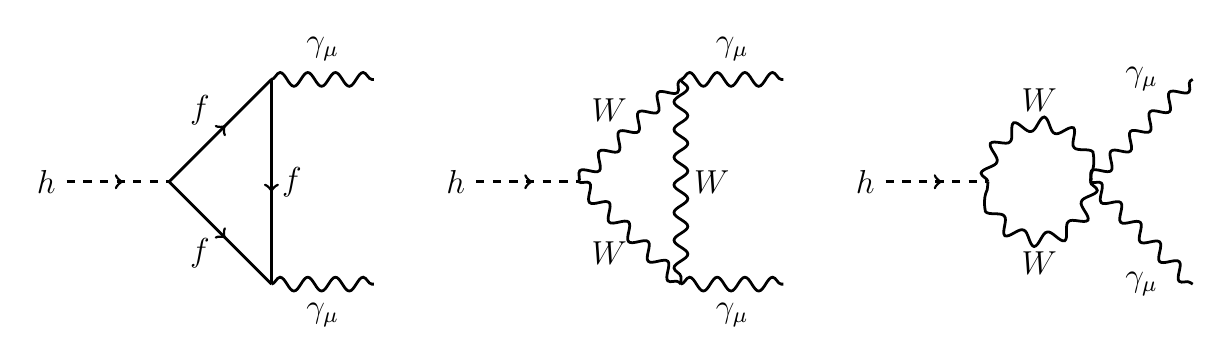
\begin{tikzpicture}[line width=1 pt, scale=1.3]
 \begin{scope}[shift={(0,0)}]
	\draw[scalar](0,0) -- (1,0);
	\draw[fermion](1,0) -- (2,1);
	\draw[fermion](1,0) -- (2,-1);
	\draw[fermion](2,1) -- (2,-1);	
	\draw[vector](2,1) --(3,1);
	\draw[vector](2,-1) -- (3,-1);
	\node at (2.5,1.3) {\large$\gamma_{\mu}$};
	\node at (2.5,-1.3) {\large$\gamma_{\mu}$};
	\node at (-0.2,0) {\large $h$};
	\node at (1.3,0.7) {\large $f$};
	\node at (1.3,-0.7) {\large $f$};
	\node at (2.2,0) {\large $f$};
 \end{scope}
\begin{scope}[shift={(4,0)}]
	\draw[scalar](0,0) -- (1,0);
	\draw[vector](1,0) -- (2,1);
	\draw[vector](1,0) -- (2,-1);
	\draw[vector](2,1) -- (2,-1);	
	\draw[vector](2,1) --(3,1);
	\draw[vector](2,-1) -- (3,-1);
	\node at (2.5,1.3) {\large$\gamma_{\mu}$};
	\node at (2.5,-1.3) {\large$\gamma_{\mu}$};
	\node at (-0.2,0) {\large $h$};
	\node at (1.3,0.7) {\large $W$};
	\node at (1.3,-0.7) {\large $W$};
	\node at (2.3,0) {\large $W$};
 \end{scope}
\begin{scope}[shift={(8,0)}]
	\draw[scalar](0,0) -- (1,0);
	\draw[vector](1,0) arc (180:0:.5);
	\draw[vector](2,0) arc (0:-180:.5);
	\draw[vector](2,0) --(3,1);
	\draw[vector](2,0) -- (3,-1);
	\node at (2.5,1) {\large$\gamma_{\mu}$};
	\node at (2.5,-1) {\large$\gamma_{\mu}$};
	\node at (-0.2,0) {\large $h$};
	\node at (1.5,0.8) {\large $W$};
	\node at (1.5,-0.8) {\large $W$};
\end{scope}
\end{tikzpicture}
\caption{Feynman diagrams which contribute to the partial width decay in the standard model.}
\end{figure}
\end{center}

\subsection{$W^{\pm}$ boson contribution}
The first diagram is
\begin{figure}[h]
\begin{center}
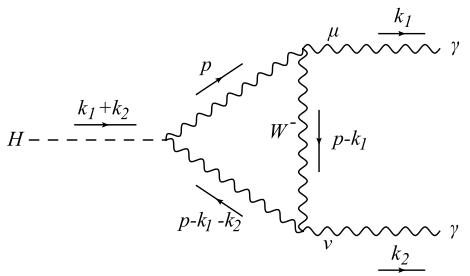
\includegraphics[scale=0.5]{./foto1.jpeg}
\end{center}
\end{figure}
\newline
Another diagram can be obtained performing an interchange of the final state photons, however  the amplitude is exactly the same as the first. Therefore we just add a factor of 2 in the first amplitude. According with the 4-momentum conservation we have
\begin{equation}
R=p-k_1 \qquad q = p-k_1-k_2
\end{equation}
Considering the Feynman rules of table 1 the matrix $\mathscr{M}_{W1}$ is
\begin{eqnarray*}
&&\mathscr{M}_{W1} = 2(igM_W g_{\alpha\alpha}) i\left(\frac{-g^{\alpha\beta} + p^{\alpha}p^{\beta}/M_W^2}{p^2-M_W^2+i\epsilon}\right) (-ie) \left[(k_1-R)^{\beta}g_{\mu\rho} + (p+R)^{\mu}g_{\rho\beta} - (p+k_1)^{\rho}g_{\mu\beta} \right]\epsilon^{\mu}(k_1) \\
&&i\left(\frac{-g^{\rho\sigma} + R^{\rho}R^{\sigma}/M_W^2}{R^2-M_W^2+i\epsilon}\right) (-ie) \left[(k_2-q)_{\sigma}g_{\nu\gamma} + (q+R)_{\nu}g_{\sigma\gamma} -(R+k_2)_{\gamma}g_{\nu\sigma} \right]\epsilon^{\nu}(k_2) i\left(\frac{-g^{\gamma\alpha} + q^{\gamma}q^{\alpha}/M_W^2}{q^2-M_W^2+i\epsilon}\right)
\end{eqnarray*}
%\newline
%\newline
The second diagram contains a 4 leg vertex where interact 2 $W$ bosons and 2 photons.
\begin{figure}[h]
\begin{center}
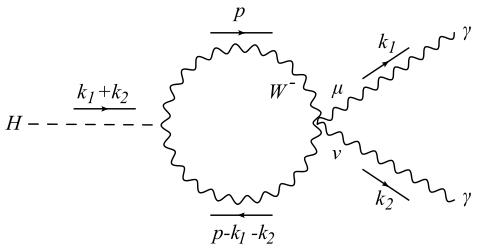
\includegraphics[scale=0.5]{./foto2.jpeg}
\end{center}
\end{figure}
\newline
%\begin{equation}
%R=p-k_1 \qquad q = p-k_1-k_2 
%\end{equation}
The matrix element of this diagram is $\mathscr{M}_{W2}$
\begin{eqnarray*}
&&\mathscr{M}_{W2} = (igM_W g_{\alpha\alpha}) i\left(\frac{-g^{\alpha\beta} + p^{\alpha}p^{\beta}/M_W^2}{p^2-M_W^2+i\epsilon}\right) (-ie^2) \left[2g_{\mu\nu}g_{\beta\gamma} - g_{\mu\beta}g_{\nu\gamma}-g_{\mu\gamma}g_{\nu\beta} \right]i\left(\frac{-g^{\gamma\alpha} + q^{\gamma}q^{\alpha}/M_W^2}{q^2-M_W^2+i\epsilon}\right)\epsilon^{\mu}(k_1)\epsilon^{\nu}(k_2)
\end{eqnarray*}

After doing the integration and adding $\mathscr{M}_{W1} + \mathscr{M}_{W2}$, we found that

\begin{eqnarray*}
&&\mathscr{M}_{W} = \frac{e^2g}{(4\pi)^2}\frac{1}{M_H^2M_W}\left[M_H^2+6M_W^2 -6M_W^2(M_H^2-2M_W^2)C_0(0,0,M_H^2,M_W^2,M_W^2,M_W^2)\right](M_H^2g^{\mu\nu}-2k_2^{\mu}k_1^{\nu})
\end{eqnarray*}

\subsection{quark top contribution}
The top contribution is
\begin{figure}[h]
\begin{center}
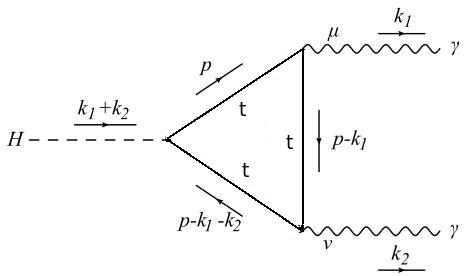
\includegraphics[scale=0.5]{./foto3.jpeg}
\end{center}
\end{figure}
\newline
Another diagram can be obtained performing an interchange of the final state photons, however  the amplitude is exactly the same as the first. Therefore we just add a factor of 2 in the first amplitude. According with the 4-momentum conservation we have
\begin{equation}
R=p-k_1 \qquad q = p-k_1-k_2
\end{equation}
Considering the Feynman rules of table 1 the matrix $\mathscr{M}_{t}$ is
\begin{eqnarray*}
\mathscr{M}_C &=& -2\frac{1}{2}ig\frac{m_t}{M_W} i \frac{(\cancel{p}+m_t)}{p^2 -m_t^2}(-ie Q_t)\gamma^{\mu} i\frac{(\cancel{R}+m_t)}{R^2 -m_t^2} (-ie Q_t)\gamma^{\nu} i \frac{(\cancel{p}+m_t)}{p^2 -m_t^2}\epsilon^{\mu}(k_1)\epsilon^{\nu}(k_2) \\
&=& ge^2Q_t^2\frac{m_t}{M_W}\frac{Tr\left[(\cancel{p}+m_t)\gamma^{\mu}(\cancel{R}+m_t)\gamma^{\nu}(\cancel{q}+m_t)\right]}{(p^2-m_t)(R^2-m_t)(q^2-m_t)}\epsilon^{\mu}(k_1)\epsilon^{\nu}(k_2)
\end{eqnarray*}




\section{VHDMM contribution}
Due to the model VHDMM contains extra vectorial particles, there is some extra diagrams which contribute to the total process.
\begin{center}
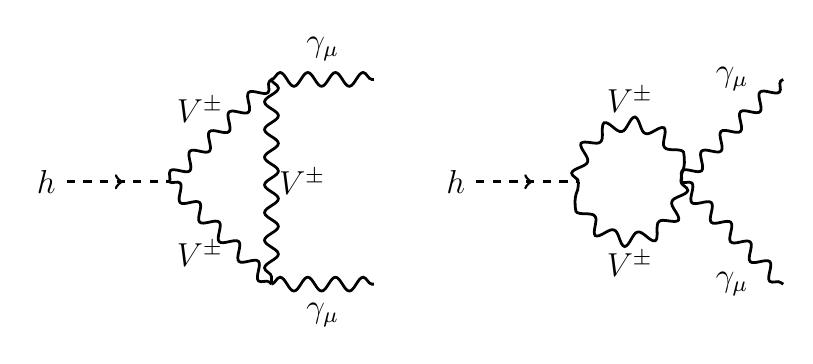
\begin{tikzpicture}[line width=1.0 pt, scale=1.3]
\begin{scope}[shift={(2,0)}]
	\draw[scalar](0,0) -- (1,0);
	\draw[vector](1,0) -- (2,1);
	\draw[vector](1,0) -- (2,-1);
	\draw[vector](2,1) -- (2,-1);	
	\draw[vector](2,1) --(3,1);
	\draw[vector](2,-1) -- (3,-1);
	\node at (2.5,1.3) {\large$\gamma_{\mu}$};
	\node at (2.5,-1.3) {\large$\gamma_{\mu}$};
	\node at (-0.2,0) {\large $h$};
	\node at (1.3,0.7) {\large $V^{\pm}$};
	\node at (1.3,-0.7) {\large $V^{\pm}$};
	\node at (2.3,0) {\large $V^{\pm}$};
 \end{scope}
\begin{scope}[shift={(6,0)}]
	\draw[scalar](0,0) -- (1,0);
	\draw[vector](1,0) arc (180:0:.5);
	\draw[vector](2,0) arc (0:-180:.5);
	\draw[vector](2,0) --(3,1);
	\draw[vector](2,0) -- (3,-1);
	\node at (2.5,1) {\large$\gamma_{\mu}$};
	\node at (2.5,-1) {\large$\gamma_{\mu}$};
	\node at (-0.2,0) {\large $h$};
	\node at (1.5,0.8) {\large $V^{\pm}$};
	\node at (1.5,-0.8) {\large $V^{\pm}$};
\end{scope}
\end{tikzpicture}
\end{center}
\end{document}

